\PassOptionsToPackage{table}{xcolor}
\documentclass[portrait,final,a0paper,fontscale=0.320]{imiseposter}
\usepackage[T1]{fontenc}
\usepackage[utf8]{inputenc}
\usepackage[ngerman]{babel}% change to ngerman for a German poster
\microtypecontext{spacing=nonfrench}
% Using biblatex and biber. It's more modern but takes more than twice as long to compile in my case. ****
% If you use biblatex, you need to comment and uncomment the marked statements in the references as well.
\usepackage{csquotes}
\usepackage[style=numeric,backend=biber]{biblatex}
\renewcommand*{\bibfont}{\tiny} % LESS SPACE FOR SOURCES
\addbibresource{poster.bib}
\addbibresource{../Dokumentation/Bibliography.bib}
%*********************************************************************************************************
\usepackage{graphicx}
\usepackage{url}% do not use hyperref as its links are displaced with baposter because of the font scale 

% PLOTS
\usepackage{float}
\usepackage{tikz}
\usepackage{pgfplots}
\pgfplotsset{compat=1.18}
\usepgfplotslibrary{groupplots}

% Select Font %%%%%%%%%%%%%%%%%%%%%%%%%%%%%%%%%%%%%%%
%\usepackage{helvet} % closest to arial
\usepackage{bookman} % has some resemblance to Futura
%%%%%%%%%%%%%%%%%%%%%%%%%%%%%%%%%%%%%%%%%%%%%%%%%%%%%
\renewcommand{\familydefault}{\sfdefault}

\newcommand{\captionfont}{\footnotesize}
\usepackage[font=small,labelfont=bf]{caption}

\begin{document}\small

\begin{poster}% Set grid to false for final print
  {grid=true,}
  % Eye Catcher
  {\hspace{3em}
\includegraphics[height=4.5cm, width=10cm, keepaspectratio]{img/logos/wog-logo-mit-text.pdf}} 
  % Title
  {Question Answering auf SNIK}
  % Authors
  {Hannes R. Brunsch\\
  Betreuer: Michael Haase, Konrad H{\"o}ffner}
  % SNIK ontology logo
  {
\includegraphics[height=9.0em]{img/logos/snik-logo.png}}

%%%%%%%%%%%%%%%%%%%%%%%%%%%%%%%%%%%%%%%%%%%%%%%%%%%%%%%%%%%%%%%%%%%%%%%%%%%%%%
\begin{posterbox}[name=background,column=0,row=0]{Hintergrund}

Das Wissen in der Medizininformatik ist sehr komplex und kompliziert.
Es liegt \textbf{in Lehrbüchern} wie etwa \cite{bb}, \cite{ob} oder \cite{he} \textbf{unstrukturiert} vor, spezifische Fragen zu beantworten kann viel Zeit kosten.
\textbf{In SNIK} liegt dieses Wissen \textbf{strukturiert} vor \cite{snik}.
Konventionelle Methoden SNIK zu durchsuchen sind jedoch sowohl in ihrer Intuitivität als auch ihrer Ausdrucksstärke mangelhaft.
Eine Lösung für dieses Problem ist \textbf{Question Answering (QA)}, die Beantwortung von in natürlicher Sprache verfassten Fragen.
Die Arbeit befasst sich mit folgendem:
\begin{enumerate}
  \item \textbf{Erstellung von Frage-Antwort-Paaren} als Benchmark und ggf. Trainingsdaten
  \item \textbf{Recherche von QA-Systemen (QASen)} sowie Evaluierung dieser anhand des Benchmarks
\end{enumerate}

\textbf{Resource Description Format (RDF)}: Darstellung von Informationen im Tripelformat \emph{Subjekt -- Prädikat --  Objekt}.
RDF ist die Modellierungssprache SNIKs.

\textbf{SPARQL Protocol and RDF Query Language (SPARQL)}: Abfragesprache für RDF.

Bei der Frage \enquote{What is the Chief Information Officer responsible for?} muss das QAS anhand der Wortgruppen \enquote{Chief Information Officer} und \enquote{is responsible for} die Antwort über eine SPARQL-Abfrage finden.
Dazu braucht es häufig \textbf{Training mittels Beispielfragen} und -antworten.

\begin{figure}[H]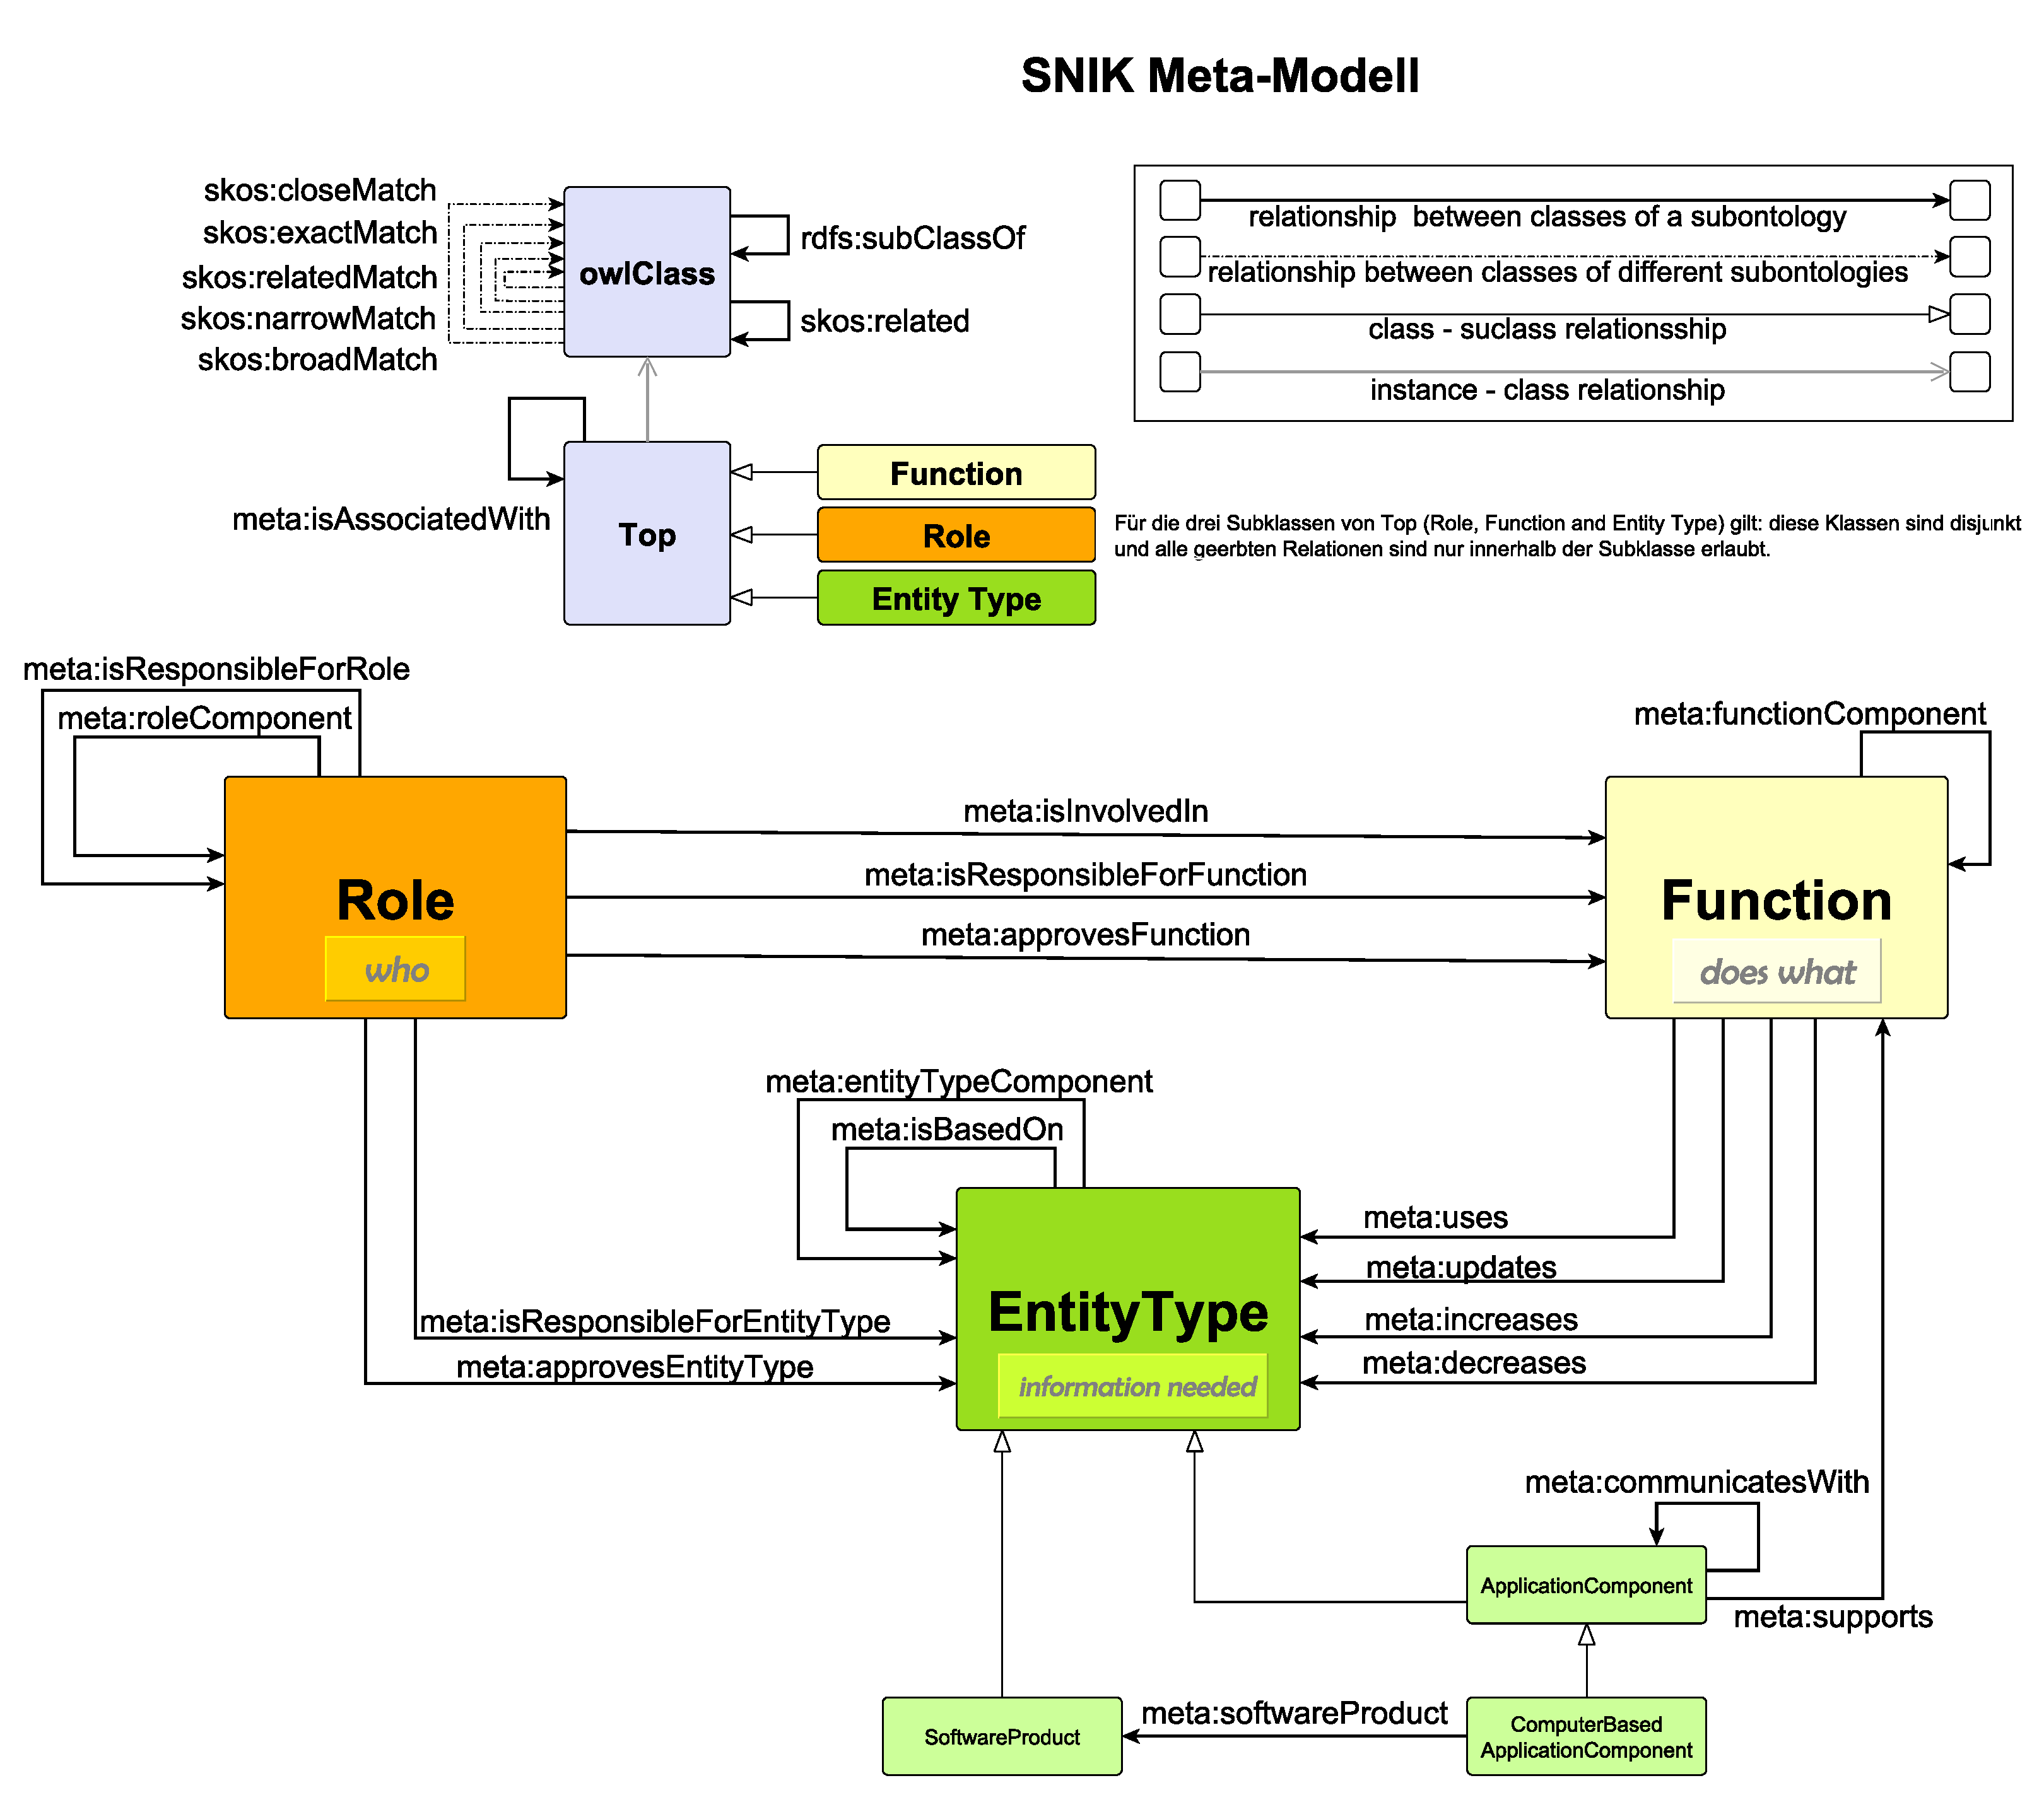
\includegraphics[width=\linewidth]{../Dokumentation/Images/snik-metamodel.pdf}\caption{Im Metamodell SNIKs ist die Metaontologie visualisiert. \small{Quelle: \protect\url{https://www.snik.eu/public/SNIK_Metamodell_V10.svg}}}\end{figure}
In SNIK wird dargestellt, \emph{wer} bezüglich Krankenhausinformationssystemen \emph{was} tut und \emph{welche Informationen} dafür benötigt werden.
Die einzelnen Quellen, aus denen SNIK sich zusammensetzt, sind in unterschiedlichen sogenannten \textbf{Teilontologien} gespeichert.

\end{posterbox}
%%%%%%%%%%%%%%%%%%%%%%%%%%%%%%%%%%%%%%%%%%%%%%%%%%%%%%%%%%%%%%%%%%%%%%%%%%%%%%
\begin{posterbox}[name=methods,below=background]{Methodik}

Es werden 995 Frage-Antwort-Paare automatisch mittels des Datensatzes generiert, 100 als \textbf{Testgruppe}, 895 als \textbf{Trainingsdaten}.
Um den Einfluss der Anzahl der Trainingsfragen auf die Leistung des QAS zu untersuchen, wird die Größe der Trainingsgruppe in Schritten von 10 erhöht.
Diese Fragen sind alle sehr \textbf{simpel}.
Es werden aus dem \textbf{Lehrbuch \cite{bb} 36 Fragen} extrahiert, welche beantwortet und zu gleichen Teilen in Trainings- und Testgruppe eingeordnet werden.
Diese sind \textbf{schwieriger}.
Es wird überprüft, ob sie sich als Trainingsfragen eignen.
Diese Arbeit \textbf{beschränkt sich auf} die das \textbf{Lehrbuch \cite{bb}} beschreibende Teilontologie.
Es werden folgende \textbf{Indikatoren} verwendet:

\textbf{Genauigkeit} (Precision): Anteil der richtigen gefundenen Antworten

\textbf{Trefferquote} (Recall): Anteil der gegebenen Antworten die richtig sind

\textbf{F-Maß} (F-Score): Harmonisches Mittel aus Genauigkeit und Trefferquote.
\end{posterbox}
%%%%%%%%%%%%%%%%%%%%%%%%%%%%%%%%%%%%%%%%%%%%%%%%%%%%%%%%%%%%%%%%%%%%%%%%%%%%%%
\begin{posterbox}[name=results,column=1]{Ergebnisse}

Als QAS wird \textbf{QAnswer KG} \cite{qanswer} ausgewählt.
Die Tests liefern folgende Ergebnisse:

% PLOTS
\begin{figure}[H]
  \begin{tikzpicture}
    \begin{groupplot}[
      group style = {
        xlabels at = edge bottom,
        ylabels at = edge left,
        horizontal sep = 2cm,
        vertical sep = 1.5cm,
        group size = 2 by 4,
      },
      width = 0.5\linewidth
      ]
      % F-Score
      \nextgroupplot[
        title=F-Maß autogenerierte Fragen,
        grid=major, % Display a grid
        grid style={dashed,gray!30}, % Set the style
        xlabel=Anzahl der generierten Trainingsfragen, % Set the labels
        ylabel=F-Maß,
        label style={font=\scriptsize},
                xtick distance=200,
                mark size=0.6,
        title style={
          at={(0.5,0.95)}, above, %yshift=0,
        },
        xmin=0,xmax=895,
        ymin=0,ymax=1,
      ]
      \addplot table[x=Anzahl Trainingsfragen,y=F-Score,col sep=comma] {../../Data/Tabellen/Training-Auswertung/generated.csv};
      \addplot table[x=Anzahl Trainingsfragen,y=F-Score,col sep=comma] {../../Data/Tabellen/Training-Auswertung/generated-withtb.csv}; 
      % F-Score TB
      \nextgroupplot[
        title=F-Maß Lehrbuchfragen,
        grid=major, % Display a grid
        grid style={dashed,gray!30}, % Set the style
        xlabel=Anzahl der generierten Trainingsfragen, % Set the labels
        ylabel=F-Maß,
        label style={font=\scriptsize},
                xtick distance=200,
                mark size=0.6,
        title style={
          at={(0.5,0.95)}, above, %yshift=0,
        },
        xmin=0,xmax=895,
        ymin=0,
      ]
      \addplot table[x=Anzahl Trainingsfragen,y=F-Score,col sep=comma] {../../Data/Tabellen/Training-Auswertung/textbook-av.csv};
      \addplot table[x=Anzahl Trainingsfragen,y=F-Score,col sep=comma] {../../Data/Tabellen/Training-Auswertung/textbook-av-withtb.csv}; 
      
      % Precision
      \nextgroupplot[
        title=Genauigkeit autogenerierte Fragen,
        grid=major, % Display a grid
        grid style={dashed,gray!30}, % Set the style
        xlabel=Anzahl der generierten Trainingsfragen, % Set the labels
        ylabel=Genauigkeit,
                label style={font=\scriptsize},
                xtick distance=200,
                mark size=0.6,
        title style={
          at={(0.5,0.95)}, above, %yshift=0,
        },
        xmin=0,xmax=895,
        ymin=0,ymax=1,
      ]
      \addplot table[x=Anzahl Trainingsfragen,y=Precision,col sep=comma] {../../Data/Tabellen/Training-Auswertung/generated.csv};
      \addplot table[x=Anzahl Trainingsfragen,y=Precision,col sep=comma] {../../Data/Tabellen/Training-Auswertung/generated-withtb.csv}; 
      % Precision TB
      \nextgroupplot[
        title = Genauigkeit Lehrbuchfragen,
        grid=major, % Display a grid
        grid style={dashed,gray!30}, % Set the style
        xlabel=Anzahl der generierten Trainingsfragen, % Set the labels
        ylabel=Genauigkeit,
        label style={font=\scriptsize},
                xtick distance=200,
                mark size=0.6,
        title style={
          at={(0.5,0.95)}, above, %yshift=0,
        },
        xmin=0,xmax=895,
        ymin=0,
      ]
      \addplot table[x=Anzahl Trainingsfragen,y=Precision,col sep=comma] {../../Data/Tabellen/Training-Auswertung/textbook-av.csv};
      \addplot table[x=Anzahl Trainingsfragen,y=Precision,col sep=comma] {../../Data/Tabellen/Training-Auswertung/textbook-av-withtb.csv}; 
      
      % Recall
      \nextgroupplot[
        title=Trefferquote autogenerierte Fragen,
        grid=major, % Display a grid
        grid style={dashed,gray!30}, % Set the style
        xlabel=Anzahl der generierten Trainingsfragen, % Set the labels
        ylabel=Trefferquote,
        label style={font=\scriptsize},
                xtick distance=200,
                mark size=0.6,
        title style={
          at={(0.5,0.95)}, above, %yshift=0,
        },
        xmin=0,xmax=895,
        ymin=0,ymax=1,
      ]
      \addplot table[x=Anzahl Trainingsfragen,y=Recall,col sep=comma] {../../Data/Tabellen/Training-Auswertung/generated.csv};
      \addplot table[x=Anzahl Trainingsfragen,y=Recall,col sep=comma] {../../Data/Tabellen/Training-Auswertung/generated-withtb.csv}; 
      % Recall TB
      \nextgroupplot[
        title=Trefferquote Textbuchfragen,
        grid=major, % Display a grid
        grid style={dashed,gray!30}, % Set the style
        xlabel=Anzahl der generierten Trainingsfragen, % Set the labels
        ylabel=Trefferquote,
        label style={font=\scriptsize},
                xtick distance=200,
                mark size=0.6,
        title style={
          at={(0.5,0.95)}, above, %yshift=0,
        },
        xmin=0,xmax=895,
        ymin=0,
        legend style={at={(-0.2,-0.3)},anchor=north}, % Put the legend below the plot
      ]
      \addplot table[x=Anzahl Trainingsfragen,y=Recall,col sep=comma] {../../Data/Tabellen/Training-Auswertung/textbook-av.csv};
      \addplot table[x=Anzahl Trainingsfragen,y=Recall,col sep=comma] {../../Data/Tabellen/Training-Auswertung/textbook-av-withtb.csv}; 
    
      % Confidence
      \nextgroupplot[
        title=Confidence autogenerierte Fragen,
        grid=major, % Display a grid
        grid style={dashed,gray!30}, % Set the style
        xlabel=Anzahl der generierten Trainingsfragen, % Set the labels
        ylabel=Confidence-Wert,
        label style={font=\scriptsize},
        xtick distance=200,
        mark size=0.6,
        title style={
          at={(0.5,0.95)}, above, %yshift=0,
        },
        xmin=0,xmax=895,
        ymin=0,ymax=1
      ]
      \addplot table[x=Anzahl Trainingsfragen,y=Confidence,col sep=comma] {../../Data/Tabellen/Training-Auswertung/generated.csv};
      \addplot table[x=Anzahl Trainingsfragen,y=Confidence,col sep=comma] {../../Data/Tabellen/Training-Auswertung/generated-withtb.csv}; 
      % Confidence TB
      \nextgroupplot[
        title=Confidence Textbuchfragen,
        grid=major, % Display a grid
        grid style={dashed,gray!30}, % Set the style
        xlabel=Anzahl der generierten Trainingsfragen, % Set the labels
        ylabel=Confidence-Wert,
        label style={font=\scriptsize},
        xtick distance=200,
        mark size=0.6,
        title style={
          at={(0.5,0.95)}, above, %yshift=0,
        },
        xmin=0,xmax=895,
        ymin=0,
        legend style={at={(-0.2,-0.3)},anchor=north}, % Put the legend below the plot
      ]
      \addplot table[x=Anzahl Trainingsfragen,y=Confidence,col sep=comma] {../../Data/Tabellen/Training-Auswertung/textbook-av.csv};
      \addlegendentry{Training ohne Lehrbuchfragen}
      \addplot table[x=Anzahl Trainingsfragen,y=Confidence,col sep=comma] {../../Data/Tabellen/Training-Auswertung/textbook-av-withtb.csv}; 
      \addlegendentry{Training mit Lehrbuchfragen}
    \end{groupplot}
  \end{tikzpicture}
  \caption{Genauigkeit, Trefferquote, F-Maß und Confidence-Wert von Lehrbuchtestfragen und automatisch generierten Testfragen in Abhängigkeit zur Anzahl und Zusammensetzung der Trainingsfragen.}
\end{figure}

\end{posterbox}
%%%%%%%%%%%%%%%%%%%%%%%%%%%%%%%%%%%%%%%%%%%%%%%%%%%%%%%%%%%%%%%%%%%%%%%%%%%%%%
\begin{posterbox}[name=discussion,column=1,below=results]{Diskussion}

Das System ist unter \url{https://app.qanswer.ai/public-share?kb=SNIK_BB&type=graph&user=kirdie&lang=en} erreichbar.
Zum Training werden 400 automatisch generierte Frage-Antwort-Paare und keine Lehrbuchfragen verwendet.
Das System liefert bei sehr einfachen Fragen ein F-Maß von $90\%$, bei Lehrbuchfragen nur etwa $25\%$.
SNIKs Eignung für QA ist aufgrund der allgemein gehaltenen Metaontologie teils fraglich.
\end{posterbox}
%%%%%%%%%%%%%%%%%%%%%%%%%%%%%%%%%%%%%%%%%%%%%%%%%%%%%%%%%%%%%%%%%%%%%%%%%%%%%%
\begin{posterbox}[name=references,column=0,below=methods]{Literatur}
    \begingroup
    \renewcommand{\section}[2]{}%suppress heading
    % using bibtex ***********
    %\bibliographystyle{abbrv}
    %\bibliography{poster}
    % using biblatex *********
    \printbibliography
    %*************************
    \endgroup
    \vspace{0.3em}
    %Myproject is supported under the DFG grant numbers 1234/5-6 and 6543/2-1.
  \end{posterbox}
%%%%%%%%%%%%%%% QAnswer Logo
\node [anchor=south east, inner sep=1pt,xshift=-10em,yshift=7em] at (current page.south east)
{
\includegraphics[height=1.5cm]{img/logos/qanswer-logo.png}};
%%%%%%%%%%%%%%% IMISE Logo
\node [anchor=south east, inner sep=1pt,xshift=-3em,yshift=1em] at (current page.south east)
{
\includegraphics[height=1.5cm]{img/logos/imise-logo.pdf}};
%%%%%%%%%%%%%%% Medical Faculty Logo
\node [anchor=south east, inner sep=1pt,xshift=-19.5em,yshift=-1.5em] at (current page.south east)
{
\includegraphics[height=3.3cm,decodearray=0 0 0 0 0 1]{img/logos/medfak.pdf}};
%%%%%%%%%%%%%%%%%%%%%%%%%%%%%%%%%%%%%%%%%%%%%%%%%%%%%%%%%%%%%%%%%%%%%%%%%%%%%%
\end{poster}
\end{document}

